\scanpage{6}
Ils correspondent aux \unsure{sous-groupes|sous-grpes} \inserted{$H$} de $\mathbb{Z}$, distincts de $\mathbb{Z}$ ($c=\operatorname{card}\mathbb{Z}/H$).....

\uline{Orientation d'un contour} : \deleted{\unsure{Ch.|En.}}

\uline{Prop} Soit\deleted{\unsure{s|x}} $X=(S,A,R)$ un contour \inserted{\deleted{\unsure{strict}}} connexe $\ne\varnothing$.

\noindent\begin{minipage}[t]{.28\linewidth}
\figure{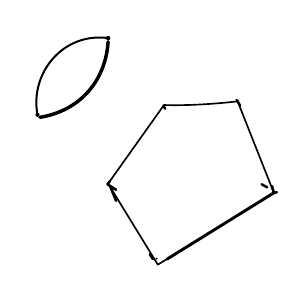
\begin{tikzpicture}[x=.0078cm,y=-.0078cm,line cap=round,line join=round]
\path[use as bounding box] (60,410) rectangle (470,810);
\draw[line width=.72pt] (76,552) .. controls (63,484) and (118,417) .. (191,427);
\draw[line width=1.25pt] (191,433) .. controls (187,495) and (147,545) .. (80,556);
\fill (76,552) circle[radius=3.4];
\fill (191,427) circle[radius=3.7];
\draw[line width=.6pt] (191,664) -- (282,536)
  .. controls (316,537) and (358,535) .. (402,530)
  -- (461,679) -- (272,796) -- cycle;
\draw[line width=1.05pt] (287,787) -- (461,679);
\draw[line width=.9pt] (194,660)--(190,665)--(204,674)
  (195,670)--(204,692)
  (281,537)--(284,542)
  (400,528)--(402,530)--(406,537)
  (458,668)--(461,679)--(466,678)
  (441,665)--(450,670)
  (259,779)--(264,787);
\fill (270,786) circle[radius=1.8];
% The detached strokes and patches are reproduced as ink, not assigned vertex or arrow semantics.
\end{tikzpicture}}
\end{minipage}\hfill
\begin{minipage}[t]{.68\linewidth}
a) \deleted{Un}\inserted{Soit $g$ un} autom. $g$ de $X$ \deleted{est dit \uline{\unsure{direct}}.}\inserted{Conditions équiv.}

\noindent\begin{tabular}{@{}l@{\quad}l@{}}
\uuline{d'orientation} & $1^{\circ})$ \deleted{si} $\forall s\in S$, $s$ est lié à $gs$ \\
 & $2^{\circ})$ $\forall a\in A\quad ga$ est lié à $a$
\end{tabular}

\deleted{\unsure{$\{$|$f$}}

\deleted{\unsure{déf.|b)}} On dit que $g$ est une \deleted{\unsure{autom.} d'}\uline{orientation} de $X$.
\end{minipage}

b) Soit $\omega(X)$\inserted{$\subset\operatorname{Aut}(X)$} l'ens des\unsure{.} \deleted{autom. d'}\unsure{orientations|orientation} de $X$

Si $g\in\omega(X)$, on a $g^{-1}\in\omega(X)$.

Alors $\operatorname{card}\omega(X)=2$ \unsure{;|,} \deleted{et si $g\in\unsure{\omega|\omega(X)}$} \inserted{(si $X$ est strict i.e. si $c=\operatorname{card}S\ne2$)} , et si $g\in\omega(X)$, on a $\omega(X)=\{g,g^{-1}\}$.

c) \deleted{Soit $\operatorname{Aut}^{+}(X)\subset\operatorname{Aut}(X)$ le ss-grpe de $\operatorname{Aut}X$ formé par les $g\in\operatorname{Aut}X$ tels que $g$ opère \unsure{triv$^{\mathrm{lt}}$|triv$^{\mathrm{t}}$} sur $\omega(X)$ [i.e.}

Considérons $\operatorname{Aut}(X)\unsure{-|\to}\operatorname{Aut}(\omega(X))\simeq\mathbb{Z}/2\mathbb{Z}$.

C'est un hom surjectif, i.e. le noyau $\operatorname{Aut}^{+}(X)$ est un ss-grpe d'indice $2$.

De plus, $\operatorname{Aut}^{\unsure{e|\varepsilon|+}}(X)$ est un groupe cyclique engendré par tt $g\in\omega(X)$.

\uline{Corollaire} $\operatorname{Aut}(X)\simeq\mathbb{Z}/2\mathbb{Z}\cdot\mathbb{Z}/H$ \inserted{(produit $\frac{1}{2}$ direct):}, où $H$ est le ss-grpe de $\mathbb{Z}$ formé des $n\in\mathbb{Z}$ tels que $g^{n}=1$ ($g$ \unsure{etant|etans|dans} une orientation fixé)
% archive sheet number: 5
